
\section{Background}\label{section:background}

\subsection{Information Retrieval (IR)}
``Information Retrieval (IR) is the activity of obtaining information resources relevant to an information need from a collection of information resources''~\cite{IR}. 
An information retrieval process begins when a user 
enters a query into the system. Queries are formal statements of information needs, for example search strings in web search engines. However, the 
submitted query may not give the satisfying results for the user. In this case, the process begins again. Figure~\ref{fig:retrieval_process} illustrates
search process.
In information retrieval, a query does not uniquely identify a single object in the collection. Instead, several objects may match the query, 
with different degrees of relevancy. In IR field, there are various types of retrieval models used to compute the degree of relevancy. This will
be discussed in more details in later section.

\begin{figure}
\centering
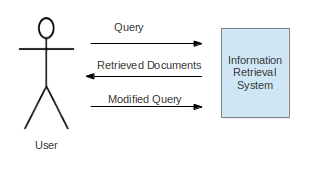
\includegraphics[scale=1]{./figures/retrieval_process.png}
\caption{Search Process} \label{fig:retrieval_process} 
\end{figure}

\subsubsection{Brief Overview of Information Retrieval System Architecture}\label{section:IRarchitecture}
In IR systems, two main objectives have to be met. First, the results must satisfy user - this means retrieving information to meet user's
information need. Second, retrieving process must be fast. This section is devoted to a brief overiew of the architecture of IR system which makes readers
understand how documents are retrieved and the data structure used in IR systems.To understand how retrieval process works, indexing process
must be understood first. This process is done offline. There are 4 steps in indexing process:
\begin{itemize}
 \item Tokenisation
 \item Stopwords Removal
 \item Stemming
 \item Index Structure Creation
\end{itemize}
Given a document containing Albert Einstein's quote about life,

\begin{quotation}
 \item There are only two ways to live your life. One is as though nothing is a miracle. The other is as though everything is a miracle.
\end{quotation}

it can be illustrated in a terms-frequency table.
\begin{figure}
\centering
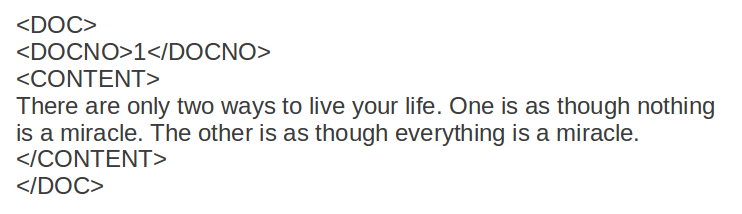
\includegraphics[scale=0.5]{./figures/text.png}
\caption{Document} \label{fig:quote} 
\end{figure}
%Figure~\ref{fig:quote} is a document containg quotes given by Albert Einstein. Figure is a table containing all the terms and 
%the frequency of each term in the document.

% 
\begin{table}
\centering
\begin{tabular}{|c|c|}

\hline \textbf{Term} & \textbf{frequency} \\
\hline there & 1 \\
\hline are & 1 \\
\hline only & 1 \\ 
\hline two & 1 \\
\hline ways & 1 \\
\hline live & 1 \\
\hline your & 1 \\
\hline life & 1 \\
\hline to & 1 \\
\hline one & 1 \\
\hline is & 3 \\
\hline as & 2 \\
\hline though & 2 \\
\hline nothing & 1 \\
\hline a & 2 \\
\hline miracle & 2 \\
\hline the & 1 \\
\hline other & 1 \\
\hline everything & 1 \\  
\hline
\end{tabular}
\caption{Terms and Frequency} \label{table:termsandfrequency}
\end{table}

Table \ref{table:termsandfrequency} shows all the terms and frequency of each term in the document. It can be seen that there are some words in the 
document which occur too frequently. These words are not good discriminators. They are referred to as ``stopwords''. They are
articles, prepositions, and conjunctions etc.

\paragraph{Tokenisation}
is the process of breaking a stream of text into words called tokens(terms). 

\paragraph{Stopwords Removal}
is the process of removing stopwords in order to reduce the size of the indexing structure. This also results in efficient lookup.
Table \ref{table:stopwordsremoval} shows all the terms and frequency of each term after stopwords removal process.

\begin{table}
\centering
\begin{tabular}{|c|c|}
\hline \textbf{Term} & \textbf{frequency} \\
\hline two & 1 \\
\hline ways & 1 \\
\hline live & 1 \\
\hline life & 1 \\
\hline one & 1 \\
\hline nothing & 1 \\
\hline miracle & 2 \\
\hline everything & 1 \\  
\hline
\end{tabular}
\caption{Terms and Frequency After Stopwords Removal} \label{table:stopwordsremoval}
\end{table}
Now, the table representing the document has shorter size and contains only meaningful words.

\paragraph{Stemming} is the process of reducing all words obtained from tokenisation process with the same root into a single root. A stem is the portion of a word which is left after
the removal of its affixes(i.e. prefixes and suffixes). For example, connect is the stem for the variants connected, connecting, and connection.
This process makes the size of the data shorter. 

\begin{table}
\centering
\begin{tabular}{|c|c|}
\hline \textbf{Term} & \textbf{frequency} \\
\hline two & 1 \\
\hline way & 1 \\
\hline live & 1 \\
\hline life & 1 \\
\hline one & 1 \\
\hline nothing & 1 \\
\hline miracle & 2 \\
\hline everything & 1 \\  
\hline
\end{tabular}
\caption{Terms and Frequency After Stemming} \label{table:stemming}
\end{table}
After stemming, all terms in the table are in its root forms. If a document is large in size, this process can reduce the size of the data. However, 
there is one drawback. That is, it prevents interpretation of word meanings. For instance, the root form of the term ``gravitation'' is ``gravity''. But
the meaning of ``gravitation'' is different from ``gravity''.

\begin{figure}
\centering
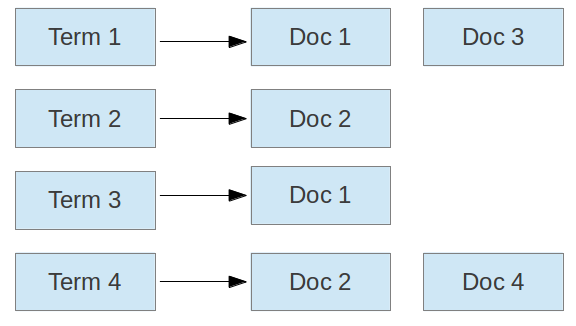
\includegraphics[scale=0.5]{./figures/invertedIndex.png}
\caption{Simple Inverted Index} \label{fig:invertedIndex} 
\end{figure}

\paragraph{Inverted Index Structure Creation} is the process that creates an index data structure storing a mapping from terms(keys) to its 
locations in a database file, or in a document or a set of documents(values)~\cite{invertedindex}. 
The purpose of this data structure is to allow a full text searches. In IR, a value in a key-value pair is called posting. 
Figure \ref{fig:invertedIndex} shows a simple inverted index. Given a query(a set of terms), it is now possible to efficiently search for
documents containing those terms. However, each posting may contain additional information about a document such as the freqency of the term etc.

\subsubsection{Retrieving results in Information Retrieval}\label{section:retrieving}
\begin{figure}
\centering
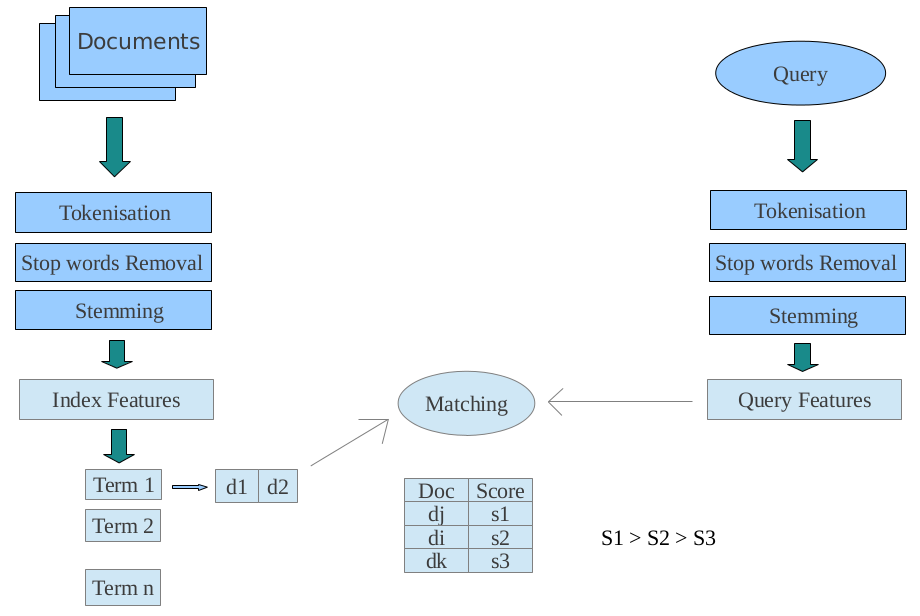
\includegraphics[scale=0.3]{./figures/retrieval.png}
\caption{Retrieval Process} \label{fig:retrieval} 
\end{figure}
Last section, basic IR systems were briefly explained. In this section, we will see how documents are retrieved. Figure ~\ref{fig:retrieval} shows
retrieval process of IR system. In IR, there are 2 phases in general:
online and offline phases. The offline phase is the phase that all documents in the corpus are indexed and all features are extracted. It begins with
tokenisation, stopwords removal and stemming as explained in the last section. Then for each document, features are extracted. The feature extracting
process is not mandatory and application dependent. One most extracted feature is the frequency of the terms occured in a document. This feature is very useful
to weight how important the document is. For instance, if a query term appears in most of the documents in the corpus, it is not appropriate to give a 
document containing that term a high score. This feature is important if an IR system uses term frequency–inverse document frequency (tf-idf) as a weighting model. But the details
of this is out of the scope of this project. Subsequently, inverted index is built.

Online phase begins after a user submits a query into the system. After that, tokenisation, stopwords removal and stemming processes are performed as same
as the offline phase. Features can also be extracted from query terms as well. At this point, it comes to the process of matching and assigning scores to documents.
Various models can be applied to obtain a score for each document. In this project, special model is used for expert search system. It will be discussed
in section ~\ref{section:voting}. Once scores have been assigned to relevant documents, the system rank all documents in order of decreasing scores and 
show to the user. Figure~\ref{fig:retrieval} gives a graphical representation of retrieval process.

\subsubsection{Evaluation}
This section is devoted to backgrounds of evaluation of IR systems. It is very important as it is a background for Evaluation Section. 
Since IR is research-based, understanding how evaluation is carried out will give a background for the readers to determine whether 
this project is achieved or not. In IR, there are 3 main reasons for evaluating IR systems~\cite[P. 3]{eval}: 
\begin{enumerate}
 \item Economic reasons: If people are going to buy the technology, they want to know how effective it is.
 \item Scientific reasons: Researchers want to know if progress is being made. So they need a measure for progress. 
	This can show that their IR system is better or worse than someone else's.
 \item Verification: If an IR system is built, it is necessary to verify the performance.
\end{enumerate}

To measure information retrieval effectiveness in the standard way, a test collection is required and it consists of 3 things~\cite{evalweb}:
\begin{enumerate}
 \item A document collection.
 \item A test suite of information needs, expressible as queries.
 \item A set of relevance judgments, standardly a binary assessment of either relevant or nonrelevant for each query-document pair.
\end{enumerate}

The standard approach to information retrieval system evaluation revolves around the notion of relevant and nonrelevant documents. With respect 
to a user information need, a document in the test collection is given a binary classification as either relevant or nonrelevant~\cite{evalweb}. However,
this can be extended by using numbers as an indicator of the degree of relevancy. For example, documents labelled 2 is more relevant than documents
labelled 1, or documents labelled 0 is not relevant. There are a number of test collection stardards. In this project, Text Retrieval Conference (TREC)
is used since it is widely used in the field of IR.

%\paragraph{Precision and Recall}
\subsubsection{Precision and Recall}
The function of an IR system is to~\cite[P. 10]{eval}:
\begin{itemize}
 \item retrieve all \textit{relevant documents} measured by \textbf{Recall}
 \item retrieve \textit{no non-relevant documents} measured by \textbf{Precision}
\end{itemize}

Precision (P) is the fraction of retrieved documents that are relevant 
\begin{center}
 \raisebox{-\totalheight}{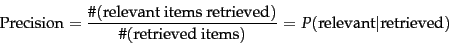
\includegraphics[scale=0.5]{./figures/precision.png}}
\end{center}

Recall (R) is the fraction of relevant documents that are retrieved 
\begin{center}
\raisebox{-\totalheight}{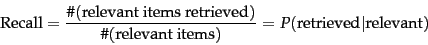
\includegraphics[scale=0.5]{./figures/recall.png}}
\end{center}

If a system has high precision but low recall, the system returns relevant documents but misses many useful ones.
If a system has low precision but high recall, the system returns most relevant documents but includes lots of junks.
Therefore, the ideal is to have both high precision and recall. To give a good example, consider Figure ~\ref{fig:pr_example}, since
overall IR system A (blue) has higher precision than IR system B (red), system A is better than system B.

\begin{figure}
\centering
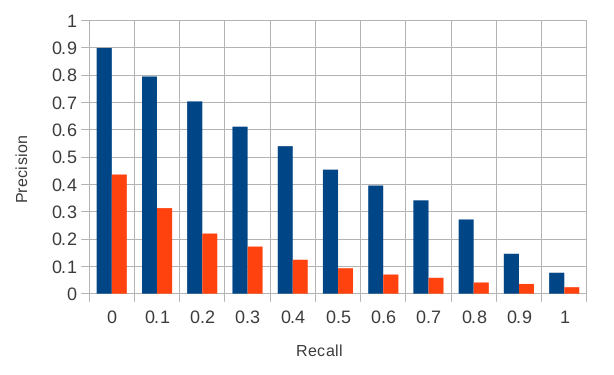
\includegraphics[scale=0.5]{./figures/pr_example.png}
\caption{Precision-Recall Graph} \label{fig:pr_example} 
\end{figure}

However, in certain cases, precisions of system A may be higher values than system B in some recall points or vice versa. Therefore,
some other measure is used instead. Most standard among the TREC community is Mean Average Precision (MAP), which provides a single-figure 
measure of quality across recall levels. This approach works by averaging all precisions. In this project, MAP is used as a measure.
\raisebox{-\totalheight}{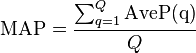
\includegraphics[scale=0.5]{./figures/map.png}}

\subsection{Search Engine}
A search engine is an information retrieval system designed to help find information stored on a computer system. The search results are usually 
presented in a list and are commonly called hits. Search engines help to minimize the time required to find information and the amount of 
information which must be consulted, akin to other techniques for managing information overload. The special kind of search engine is 
web search engine. It is a software system that is designed to search for information on the World Wide Web.

\subsection{Learning to Rank}
Learning to rank or machine-learned ranking (MLR) is a type of supervised or semi-supervised machine learning problem in which the goal is 
to automatically construct a ranking model from training data~\cite{letor}. Ranking is the central problem for information retrieval. 
However, employing learning to rank techniques to learn the ranking function is viewed as
a promising approach to information retrieval~\cite{letor}. In particular, many learning to rank aproaches attempt to learn a combination of features
(called the learned model)~\cite[P. 3]{learningmodel}. The resulting learned model is applied to a vector of features for each document, to determine the final scores for 
producing the final ranking of documents for a query~\cite[P. 3]{learningmodel}. In learning to rank, a feature is a binary or numberical indicator 
representing the quality of a document, or its relation to the query~\cite[P. 4]{learningmodel}. This will be discussed in more details in later section.

\subsubsection{Query Dependent Feature}\label{section:querydependent}
Figure~\ref{fig:retrieval_process} shows a simple search process in IR. After a user submits a query into an IR system. The system ranks the results 
with respect to the query and returns a result set to the user. It can be clearly seen that the results obtained with respect to the query depends on the 
query the user submitted. In other words, document A can have 2 different degrees of relevancy if a user changes a query.
In learning to rank, this is called query dependent feature.

\subsubsection{Query Independent Feature}\label{section:queryindependent}
In contrast to Query Dependent Feature, a feature that does not depend on a user query is called query independent feature. This feature is fixed for each
document. For now, it is better to not dig into great details about this because this will be focused in later section.

\subsubsection{Obtaining and Deploying a Learned Model} \label{section:learnedmodel}
The general steps for obtaining a learned model using a learning to rank technique are the following~\cite[P. 4]{learningmodel}:

\begin{quote}
  \item 1. Top k Retrieval: For a set of training queries, generate a sample of k documents using an initial retrieval approach.
  \item 2. Feature Extraction: For each document in the sample, extract a vector of feature values. 
  \item 3. Learning: Learn a model by applying a learning to rank technique. Each technique deploys a different loss function to estimate the goodness of
	various combination of features. Documents are labelled according to available relevance assessments.

Once a learned model has been obtained from the above learning steps, it can be deployed within a search engine as follows~\cite[P. 4]{learningmodel}

 \item 4. Top k Retrieval: For an unseen test query, a sample of k documents is generated in the same manner as step (1).
 \item 5. Feature Extraction: As in step (2), a vector of feature values is extracted for each document in the sample. The set of features should be exactly
	the same as for (2).
 \item 6. Learned Model Application: The final ranking of documents for the query is obtained by applying the learned model on every document in the sample,
	and sorting by descending predicted score.
\end{quote}

\begin{figure}
\centering
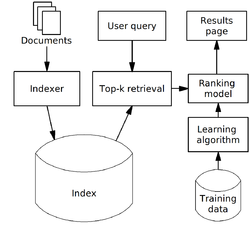
\includegraphics[scale=0.7]{./figures/letor.png}
\caption{An architecture of a machine-learned IR system from \protect\url{http://en.wikipedia.org/wiki/Learning_to_rank}} \label{fig:letor} 
\end{figure}
Figure~\ref{fig:letor} illustrates an architecture of a machine-learned IR system. The architecture will be discussed in more details in Design and 
Implementation Section.

\subsection{Tools}
\subsubsection{Terrier}\label{section:terrier}
Every IR system requires programs that handle indexing, retrieving, ranking, etc. To build everything from scratch, it would be impossible within
the time range. However, there are a number of search engine platforms that deal with IR functionalities effectively.
Terrier~\cite{terrier} is a highly flexible, efficient, and effective open source search engine, readily deployable on large-scale collections of documents. 
Terrier implements state-of-the-art indexing and retrieval functionalities, and provides an ideal platform for the rapid development and evaluation 
of large-scale retrieval applications. It is open source, and is a comprehensive, flexible and transparent platform for research and 
experimentation in text retrieval. Research can easily be carried out on standard TREC and CLEF test collections.

\subsubsection{RankLib}\label{section:rankLib}
RankLib~\cite{ranklib} is an open source library of learning to rank algorithms. It also implements many retrieval metrics as well as provides many ways to carry out evaluation.
Currently eight popular algorithms have been implemented:
\begin{itemize}
 \item MART (Multiple Additive Regression Trees, a.k.a. Gradient boosted regression tree)
 \item RankNet
 \item RankBoost
 \item AdaRank
 \item Coordinate Ascent
 \item LambdaMART
 \item ListNet
 \item Random Forests
\end{itemize}

However, AdaRank and Coordinate Ascent are only used in the project because other algorithms are too complex and not part of the scope of this project.

\subsubsection{trec\_eval}
trec\_eval is the standard tool used by the TREC community for evaluating a retrieval run, given the results file and a
standard set of judged results. 

\subsection{Expert Search}
\subsubsection{Determining Good Query Results}
Figure~\ref{fig:retrieval_process} illustrates the process of search. From this figure, the process will start again if a user is not satisfied with 
the results. In this section, the focus is on how to convince user that a query result is good. Suppose a user who is currently studying software engineering
would like to know ``how to normalize database tables'', first of all, he needs to interpret his information need into a query which is ``database normalization''.
He then types his query into his preferred search engine. After he submits the query, the search engine gives him a list of results ranked by the degree
of relevancy. The question is how does he determine which result is what he is looking for?. Well, he could assume that the ranking provided by the search 
engine is correct. That is, the first result is what he is looking for. However, this is not always the case. He then explores each result and sees if 
it is the right one. But without exploring each result, could he be able to determine that which result is likely to satisfy his information need?
Perhaps, there has to be some evidence to convince him by just looking at the result. The followings are evidence he could take into account~\cite{craig}: 
\begin{itemize}
 \item URL
 \item Photo
 \item Author
 \item keywords of the article name
\end{itemize}
If a result in response to a query have all or some of these evidence, it has more credits than ones with no evidence at all. 
\begin{figure}
\centering
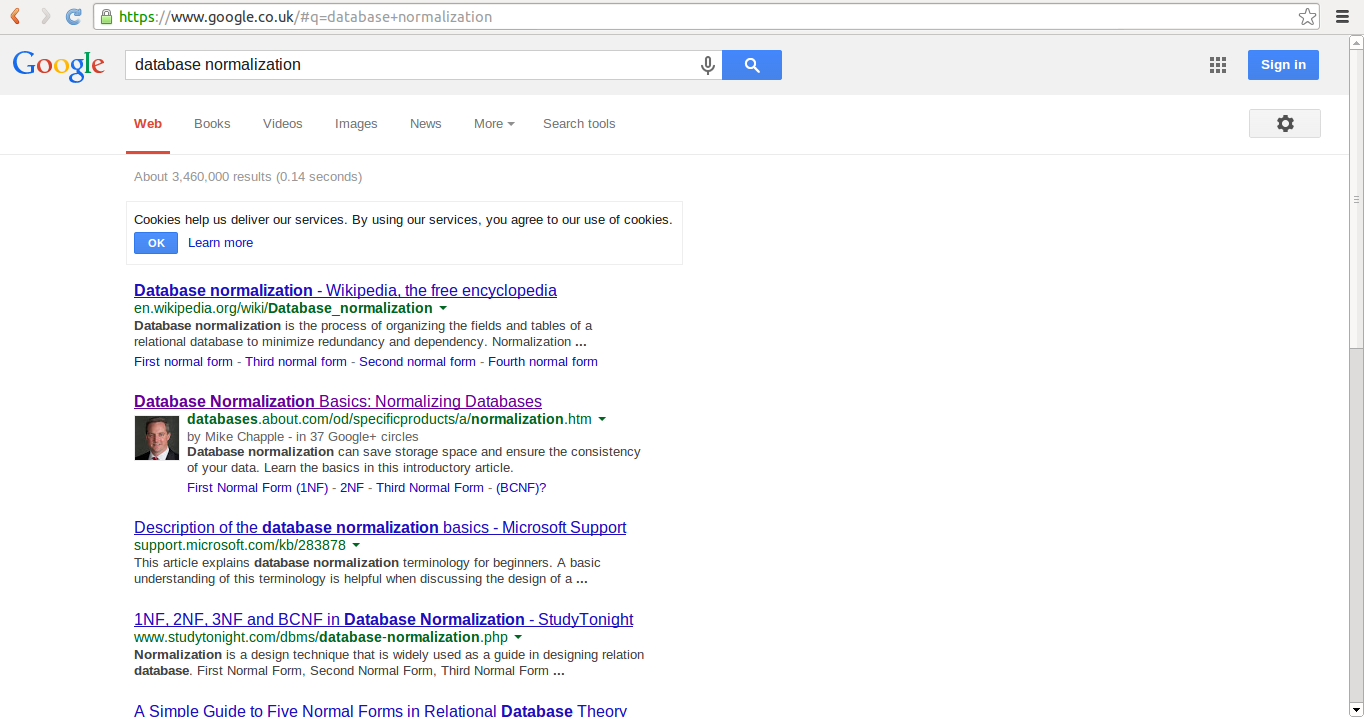
\includegraphics[scale=0.3]{./figures/query.png}
\caption{Sample Query} \label{fig:query}
\end{figure}
Figure \ref{fig:query} shows the results of the query ``database normalization''. It is obvious that from the top 4 results, all of the article names
include the keywords a user submitted, and the third result does not have query keywords included in the URL. Among all of which, the second result has more 
evidence than others. It has an author's name, a photo of an author that other results do not.

\subsubsection{What makes an expert a good expert?}\label{section:goodexpert}
Last section, it was obvious that some evidence could be used to convince users how reliable a document (link) is. In this secion, the evidence within
the context of this project will be discussed. As discussed in ~\ref{section:aims}, this project makes use of publications and funded projects as 
expertise evidence. Based on these evidence, what makes an expert a good expert? Well, it is common sense to assume that an expert is professional if 
\begin{itemize}
 \item he has published a lot of publications.
 \item he has co-authored with a lot of other experts in publications.
 \item he has co-authored with a lot of other experts in funded projects.
 \item he has received a lot of funding.
 \item he has involved in a lot of projects.
\end{itemize}

It can be seen clearly that these assumptions or features in learning to rank are independent on the query a user submits. These features are query independent
(section ~\ref{section:queryindependent}). However, query dependent features (section~\ref{section:querydependent}) should take into account as well. 
In this project, there are 2 query dependent features: funded project and publication features. To sum up, a good expert should have high scores in
both query dependent and independent features.

\subsubsection{Voting Technique}\label{section:voting}
In section ~\ref{section:retrieving}, we very briefly talked about weighting model. In other words, how documents are assigned scores using tf-idf. In this section,
it aims to give an overview of voting technique used in this project. To understand this section, readers must understand what data fusion technique is. 
``Data fustion techniques also known as metasearch techniques, are used to combine separate rankings of documents into a single ranking,
with the aim of improving over the performance of any constituent ranking''~\cite[P. 388]{expertsearch}. Within the context of this project, 
expert search is seen as a voting problem. The profile of each candidate is a set of documents associated to him to represent their expertise.
When each document associated to a candidate's profile get retrieved by the IR system, implicit vote for that candidate occurs~\cite[P. 389]{expertsearch}.
Data fusion technique is then used to combine the ranking with respect to the query and the implicit vote. In expert search task, it shows that 
``improving the quality of the underlying document representation can significantly improve the retrieval performance of the data fusion techniques 
on an expert search task''~\cite[P. 387]{expertsearch}. To give a simple example how data fusion technique works, take a look at this example

Let R(Q) be the set of documents retrieved for query Q, and the set of documents belonging to the profile candidate C be denoted profile(C). In expert
search, we need to find a ranking of candidates, given R(Q). Consider the simple example in Tables ~\ref{table:ranking} and ~\ref{table:profiles}.
The ranking of documents with respect to the query has retrieved documents \{D1, D2, D3, D4\}. Using the candidate profiles, candidate C1 has accumulated
3 votes, C2 2 votes, C3 2 votes and C4 no votes. If all votes are counted equally, and each document in a candidate's profile is equally weighted, a possible
ranking of candidates to this query could be \{C1, C2, C3\}. However, in this project, the technique used is expCombMNZ and the formular is as follows

\begin{table}
\centering
\begin{tabular}{|c|c|c|}
\hline \textbf{Rank} & \textbf{Docs} & \textbf{Scores}\\
\hline 1 & D1 & 5.4 \\
\hline 2 & D2 & 4.2\\
\hline 3 & D3 & 3.9 \\
\hline 4 & D4 & 2.0 \\  
\hline
\end{tabular}
\caption{R(Q)} \label{table:ranking}
\end{table}
\quad
\begin{table}
\centering
\begin{tabular}{|c|l|}
\hline \textbf{Profiles} & \textbf{Docs}\\
\hline C1 & D3, D4, D2 \\
\hline C2 & D1, D2 \\
\hline C3 & D3, D2 \\
\hline C4 & D5, D6 \\  
\hline
\end{tabular}
\caption{Profiles} \label{table:profiles}
\end{table}

\[
candScore(C,Q) = |R(Q) \cap profile(C)| \sum_{d \in R(Q) \cap profile(C)} score_d
\]
where \[|R(Q) \cap profile(C)|\] is the number of documents from the profile of candidate C that are in the ranking R(Q).














